\thesolution{Coda a Priorit�}
Si vuole una coda in cui gli elementi possano essere liberamente accodati e siano connotati da uno tra due possibili livelli di priorit�. Il prelievo di un elemento dalla coda dovr� rispettare, in primis, il livello di priorit� e, nell'ambito degli elementi aventi la stessa priorit�, la disciplina \emph{first-in-first-out} (FIFO) di una coda.

La traccia specifica esclusivamente il comportamento ``esteriore'' della struttura dati, senza definire alcun dettaglio di natura implementativa. Per ottenere una struttura avente il comportamento specificato � possibile seguire diverse strade. Di seguito sono riportate alcune possibilit�.

\subsection*{Approccio 1}
La coda a priorit� pu� essere immaginata formata da una sequenza di elementi costituita a sua volta da due sotto-sequenze (\seename\ \figurename~\ref{fig:SottoSequenze}):
\begin{itemize}
\item una prima sotto-sequenza, che parte dalla testa, che comprende gli elementi a priorit� alta;
\item una successiva sotto-sequenza, che si estende fino alla coda, che comprende gli elementi a priorit� bassa.
\end{itemize}
Una o entrambe queste sotto-sequenze possono in generale essere vuote.

Dal momento che le operazioni di prelievo (\cod{pop()}) e di inserimento a bassa priorit� (\cod{pushLow()}) corrispondono in questo caso alle normali operazioni usate nel caso di una classica coda, l'unica operazione nuova da implementare consiste nell'inserimento in coda di un elemento a priorit� alta (\cod{pushHigh()}). Tale operazione prevede l'aggiunta di un elemento ``in coda'' agli elementi a priorit� alta. In quest'ottica risulta utile definire un puntatore \cod{h} aggiuntivo posizionato sull'ultimo degli elementi a priorit� alta.
Tale nuovo puntatore punter� alla coda degli elementi ad alta priorit�, oppure varr� \cod{null} in caso di assenza di tali elementi.

\begin{figure}
  \center
	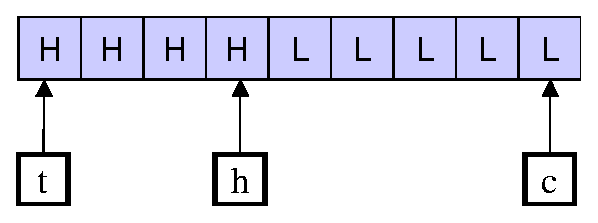
\includegraphics[width=.5\textwidth]{Esercizi/CodaAPriorita/2.eps}
	\caption{Una sequenza di elementi formata da due sotto-sequenze consecutive}
	\label{fig:SottoSequenze}
\end{figure}

\inputmodule{PriorityQueue.java}{Esercizi/CodaAPriorita/1/PriorityQueue.java}

\subsection*{Approccio 2}
La coda a priorit� pu� essere immaginata composta di due classiche code affiancate (\seename\ \figurename~\ref{fig:CodeAffiancate}), ciascuna destinata a contenere gli elementi di una singola classe. Il metodo \cod{pushLow()} accoda nella coda a bassa priorit�. Il metodo \cod{pushHigh()}, viceversa, in quella ad alta priorit�. Il metodo \cod{pop()} restituisce l'elemento di testa nella coda ad alta priorit�, se esiste; in caso contrario restituisce l'elemento di testa nella coda a bassa priorit�.

Servendosi del meccanismo dell'aggregazione stretta tra classi, le due code affiancate risultano istanze della classe \cod{Coda} (\cfr{Ex:Coda}). Definendo tali istanze come membri privati della classe \cod{PriorityQueue} esse non risulteranno visibili dall'esterno della struttura (\emph{information hiding}), la quale continuer� ad apparire ai suoi utenti come una singola coda dotata dei meccanismi di priorit� richiesti.

\begin{figure}
  \center
	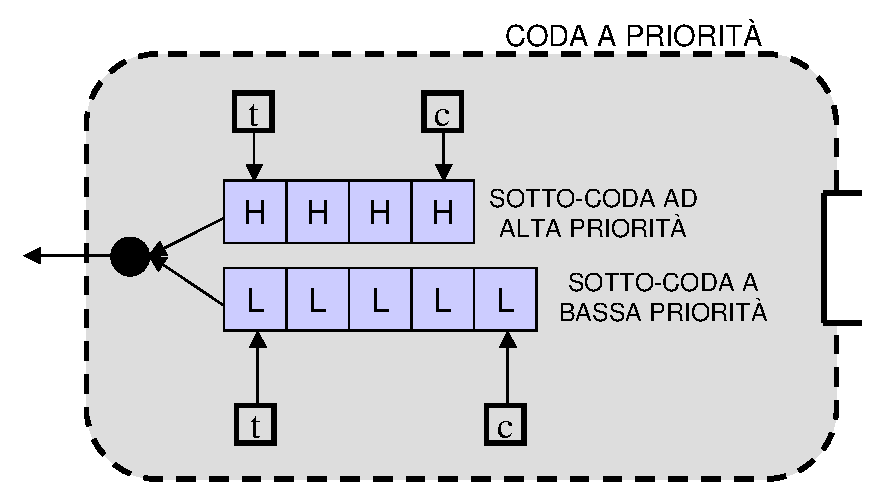
\includegraphics[width=.7\textwidth]{Esercizi/CodaAPriorita/4.eps}
	\caption{Coda a priorit� formata da due classiche code affiancate}
	\label{fig:CodeAffiancate}
\end{figure}

\inputprogram{Esercizi/CodaAPriorita/2/PriorityQueue.java}

\subsection*{Approccio 3}
La coda a priorit� pu� essere una normale coda in cui i record, disposti secondo l'ordine di inserimento, vengono etichettati con la loro priorit�\footnote{Questo � possibile previa definizione di un'opportuna classe che contenga un elemento \cod{int} ed un valore \cod{boolean} indicante la relativa priorit�.} (\seename\ \figurename~\ref{fig:ElementiEtichettati}). In questo caso sia il metodo \cod{pushHigh()} che il metodo \cod{pushLow()}, previa opportuna etichettatura, effettuano un'aggiunta in coda. \`E il metodo \cod{pop()} in questo caso a prendersi carico della restituzione del ``giusto'' elemento. Tale operazione viene effettuata scorrendo tutta la struttura alla ricerca del primo elemento ad alta priorit� e restituendolo dopo averlo eliminato dalla coda. In assenza di un elemento ad alta priorit� viene restituito l'eventuale elemento di testa.

\begin{figure}
  \center
	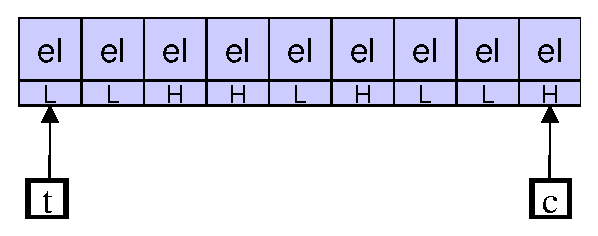
\includegraphics[width=.5\textwidth]{Esercizi/CodaAPriorita/3.eps}
	\caption{Sequenza di elementi ``etichettati''}
	\label{fig:ElementiEtichettati}
\end{figure}

Tale implementazione, pur prestandosi a diverse ottimizzazioni, non risulta particolarmente efficiente, richiedendo un ciclo di ricerca per ogni operazione \cod{Pop()} effettuata. La sua implementazione non � qui riportata.

Si riporta invece l'implementazione della classe Main che usa una qualsiasi delle due implementazioni presentate di sopra, proprio perch� queste sono compatibili a livello di interfaccia.

\inputprogram{Esercizi/CodaAPriorita/1/Main.java}